\documentclass[12pt,a4paper]{article}

\setlength{\parskip}{\baselineskip} % Increase space between paragraphs
\setlength{\parindent}{0pt} % No indentation at paragraph level

\renewcommand{\familydefault}{cmss}
\newcommand{\rp}{\textbf{Raspberry Pi}\xspace}

\usepackage{xspace}
\usepackage[ngerman]{babel} % This is needed for umlauts
\usepackage[utf8]{inputenc} % This is needed for umlauts
\usepackage[T1]{fontenc} % This is needed for correct output of umlauts in pdf
\usepackage[pdftex,breaklinks,colorlinks,
citecolor=blue,
urlcolor=blue]{hyperref}
\usepackage{graphicx}
\usepackage[german]{cleveref} % Prepend \ref with corresponding label
% Use smaller margins
\usepackage[cm]{fullpage}
\usepackage{layout}
\usepackage{float}
\usepackage{wrapfig}
\usepackage{textcomp}
\usepackage{eurosym}

% 'graphicx' configuration
\graphicspath{ {img/} }
\DeclareGraphicsExtensions{.jpg}

% Copy title, author to PDF metadata
\makeatletter
\AtBeginDocument{
  \hypersetup{
    pdftitle = {\@title},
    pdfauthor = {\@author}
  }
}
\makeatother

\begin{document}
% '\layout' to visualize the layout applied
\title{Raspberry Pi}
\author{Hr. Walter, Hr. Ehret und Hr. Ribeaud}
\maketitle

Die \rp Hardware ist ein Einplatinen Computer der von der britischen \href{https://www.raspberrypi.org/}{Raspberry Pi Foundation} gefertigt wird.

Der \rp wurde 2008 ursprünglich entwickelt, Kinder spielerisch in die Welt der Programmierung \& Elektronik einzuführen. Jedoch führte die einfache Handhabung und die fast unendlichen Möglichkeiten zu einer grossen Community, die mittlerweile durch alle Schichten und Altersklassen geht.

Der Name wird wie \textit{raspberry pie} ausgesprochen, das englische Wort für Himbeerkuchen. Die \textit{Himbeere} knüpft an die Tradition an, Computer nach Früchten zu benennen, wie etwa \textbf{Apple}. Das \textbf{Pi} stammt aus \textit{Python}, einer Programmiersprache.

Bis Februar 2017 wurden mehr als zwölf Millionen Geräte verkauft. Die Entwicklung des \textbf{Raspberry Pi} wurde mit mehreren Auszeichnungen bzw. Ehrungen bedacht. Es existiert ein großes Zubehör- und Softwareangebot für zahlreiche Anwendungsbereiche. Verbreitet ist beispielsweise die Verwendung als \href{https://www.youtube.com/watch?v=YPu7oSVbMVo}{Mediacenter}, da der Rechner Videodaten mit voller HD-Auflösung (1080p) dekodieren und über die HDMI-Schnittstelle ausgeben kann. 

\section{Anschlüsse und Komponenten}
\label{sec:comp}

Bevor man mit dem \rp richtig loslegen kann, muss man zumindest grob wissen, wo welche Anschlüsse und Komponenten liegen und für was sie gut sind. Deshalb gilt es, alle wichtigen Anschlüsse und Bauteile des \rp richtig zu identifizieren.

\subsection{Aufgabe}

Auf dem unteren Foto des \rp zeichne die folgenden Anschlüsse und Komponenten ein. Antwort befindet sich im \cref{apx:comp} (\cref{fig:rp_ls}).

\begin{figure}[H]
\centering
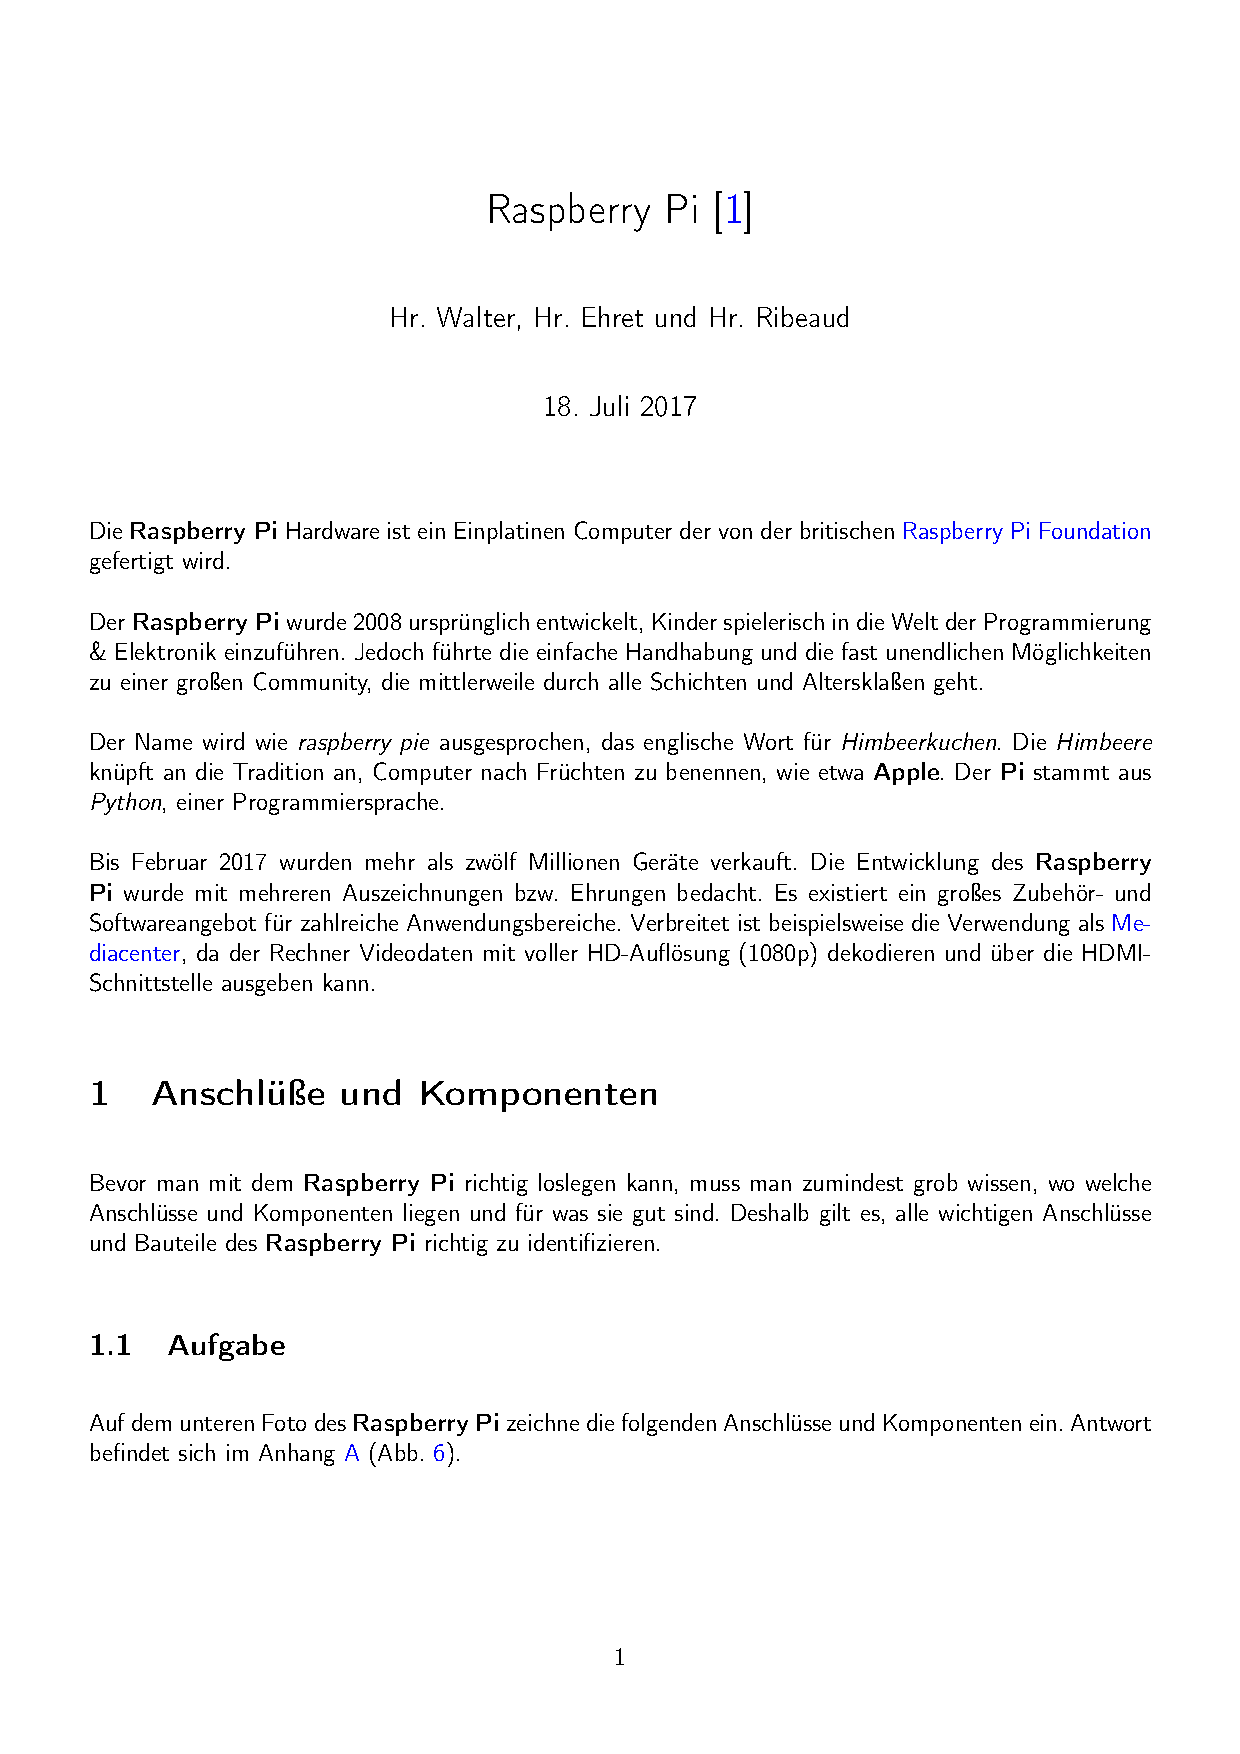
\includegraphics[scale=1.3]{raspberry}
\caption{Raspberry Pi 3}
\label{fig:rp}
\end{figure}

\begin{enumerate}
\item Wo befindet sich der Tastatur- und Maus-Anschluss (USB)?
\item Wo befindet sich der Netzwerk-Anschluss (Ethernet)?
\item Wo befindet sich der Anschluss für einen Bildschirm (HDMI)?
\item Wo befindet sich der Anschluss für Lautsprecher (Klinke)?
\item Wo befindet sich der Anschluss für die Energieversorgung (Micro-USB)?
\item Wo befindet sich der Steckplatz für die SD-Speicherkarte?
\item Wo befindet sich der Steckplatz für Erweiterungen (GPIO)?
\end{enumerate}

\section{Was man noch braucht}
\label{sec:acc}

\subsection{SD Karte}

\begin{wrapfigure}{r}{0.2\textwidth}
  \vspace{-25pt}
  \begin{center}
    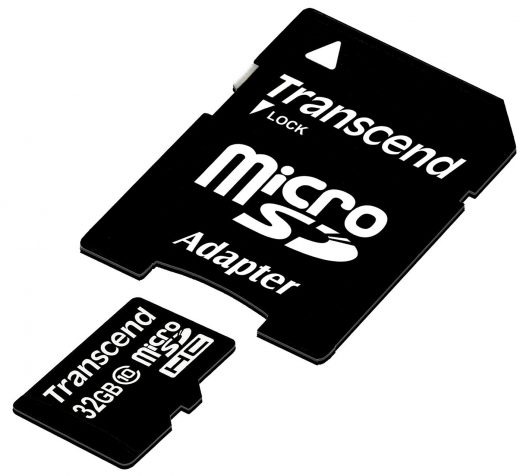
\includegraphics[scale=0.2]{sd_card}
  \end{center}
  \vspace{-25pt}
\end{wrapfigure}

Die \textbf{SD Karte} ist essenziell, denn das \rp kann nicht von einem USB Stick oder Festplatte gestartet werden. Der Geschwindigkeit halber wird eine \textit{Class 10 SD} mit mindestens \textit{8 GB} Kapazität empfohlen. Prinzipiell sind aber bis zu 32 GB möglich. Die minimal benötigte Größe variiert von Betriebssystem zu Betriebssystem zwischen 2 und 6 GB. Falls man eine alte (micro)SD Karte aus der Kamera oder dem Handy hat, kann man diese benutzen.

\subsection{Stromversorgung}

\begin{wrapfigure}{r}{0.2\textwidth}
  \vspace{-12pt}
  \begin{center}
    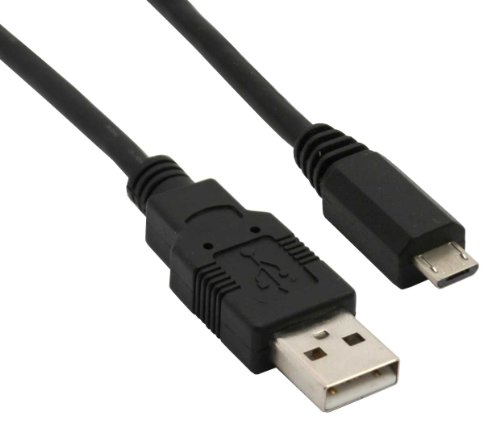
\includegraphics[scale=0.2]{microusb}
  \end{center}
  \vspace{-25pt}
\end{wrapfigure}

Damit der \textbf{Pi} genug Strom bekommt, braucht man ein \textbf{microUSB Kabel} mit Netzteil (gibt es auch in einem). Wenn man bereits ein \textbf{microUSB Kabel} hast, braucht man nur noch ein USB Netzteil, welches für den Dauerbetrieb geeignet ist und mindestens \textit{1000mA} liefert (auch diese sind separat erhältlich). Das Raspberry Pi 2/3 sollte mit einem Netzteil, welches \textit{2000mA} liefert an den Strom angeschlossen werden.

\subsection{HDMI Kabel}

\begin{wrapfigure}{r}{0.2\textwidth}
  \vspace{-30pt}
  \begin{center}
    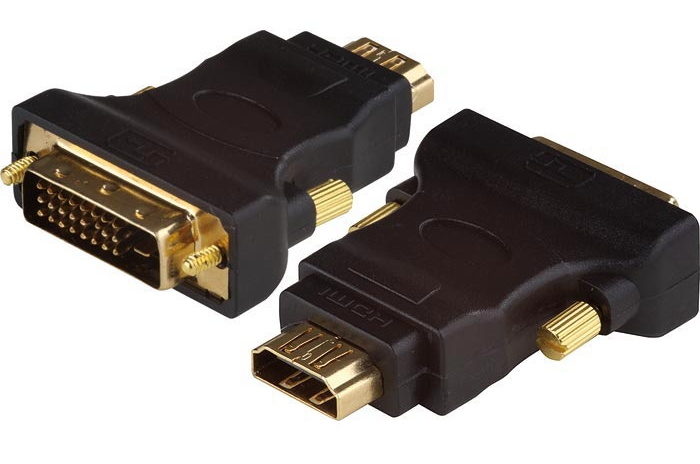
\includegraphics[width=3cm]{hdmi}
  \end{center}
  \vspace{-25pt}
\end{wrapfigure}

Das \textbf{HDMI Kabel} dient dazu, einen Bildschirm anzuschliessen. Wenn der Bildschirm über keinen HDMI Anschluss verfügt (\textbf{DVI} od. \textbf{VGA}), dann muss man sich einen Adapter besorgen.

\subsection{Maus und Tastatur}

\textbf{Maus} und \textbf{Tastatur} werden via USB angeschlossen.

\subsection{Gehäuse}

Da der \textbf{Pi} ohne Zubehör, also auch ohne äußere Verkleidung geliefert wird, kann man ein Gehäuse nachkaufen. Es gibt sie in verschiedenen Formen und Farben (ab 3€ aufwärts). Unbedingt notwendig ist es aber nicht, daher sollte jeder für sich selbst entscheiden, ob er eines benötigt oder nicht.

Was allerdings sehr empfehlswert ist, vor allem wenn der \textbf{Pi} dauerhaft oder längere Zeit laufen soll, sind Kühlkörper. Ein Set besteht aus 3 Kühlkörpern, für die verschiedenen Chips des \textbf{Pi}'s. Zwar sind die Chips des Raspberry’s so gemacht, dass sie nicht überhitzen (wie bspw. der Prozessor im Handy), aber dennoch kann die CPU bis zu 45° heiß werden, was nicht besonders zur Langlebigkeit beiträgt. Wer beides will, kann auch einfach auf ein Gehäuse mit Kühlkörpern dabei zurückgreifen.

\section{Hardware}

\subsection{GPIO}

\textbf{GPIO} steht für \textit{General Purpose Input/Output}. Über diese Schnittstelle können diverse Geräte angesteuert werden (LEDs, Sensoren, Displays, etc).

\begin{figure}[H]
\centering
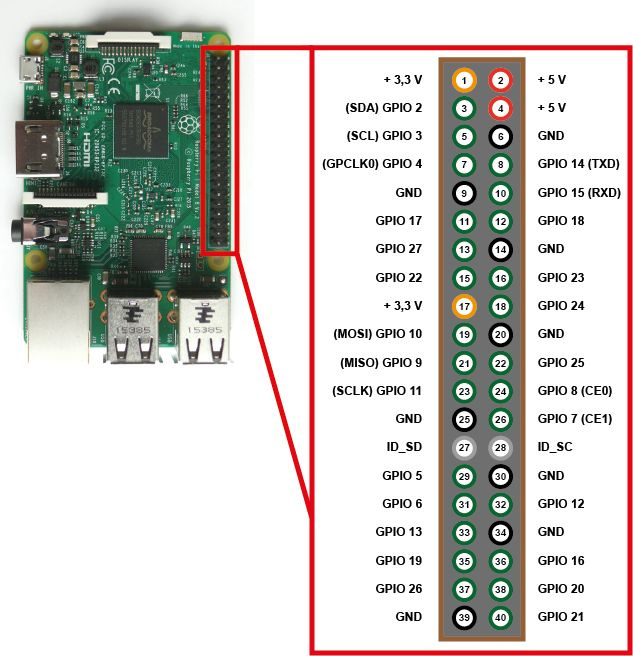
\includegraphics[scale=.5]{gpio}
\caption{General Purpose Input/Output}
\label{fig:gpio}
\end{figure}

\subsection{CSI}

Das \textbf{CSI} erlaubt die direkte Anbindung einer Kamera. Das \textit{Camera Serial Interface} kann eine Kamera mit 5MP ansteuern. Fotos oder Videos sind in diversen Auflösungen möglich.

\begin{figure}[H]
\centering
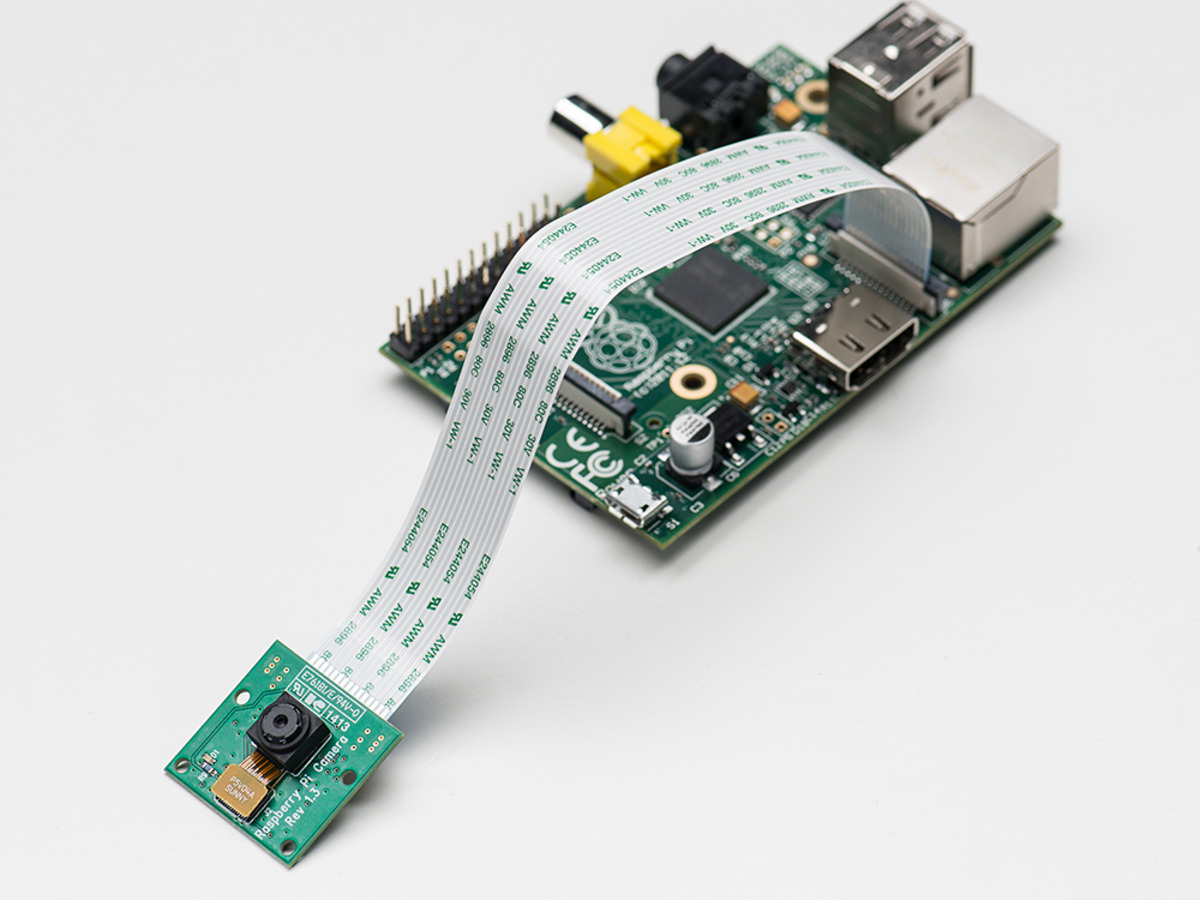
\includegraphics[scale=.8]{csi}
\caption{Camera Serial Interface}
\label{fig:gpio}
\end{figure}

% Wie sieht aus, sobald wir uns eingeloggt haben?

\clearpage
\appendix
\makeatletter
\def\@seccntformat#1{Anhang~\csname the#1\endcsname:\quad}
\makeatother

\section{Anschlüsse und Komponenten}
\label{apx:comp}

\begin{figure}[h]
\centering
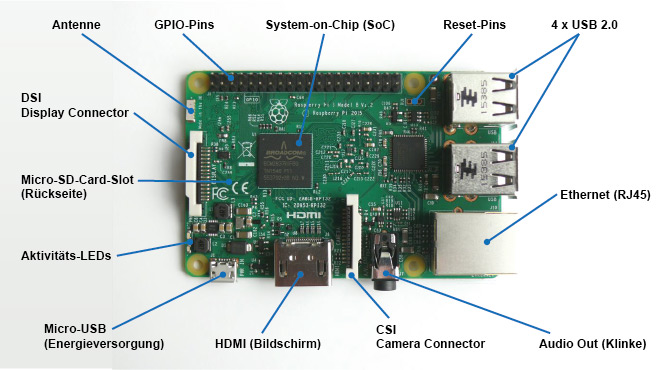
\includegraphics[scale=0.7]{raspberry_loesung}
\caption{Raspberry Pi 3}
\label{fig:rp_ls}
\end{figure}

\end{document}
